We identified three previously existing resources that can be of use for analysis and modeling of object naming: RefCOCO (and a variant, RefCOCO+), Flickr30k Entities, and Visual Genome. Table~\ref{tab:compare} summarizes their main characteristics and compares them to our dataset (last two columns; see Section~\ref{+++}). 
As the table shows, previous datasets provide between one and three annotations per object, which, we believe, is not enough to examine naming variation.
This motivates our data collection, in which we collect 36 names per object.
Still, because these datasets can be useful to examine other aspects of object naming, and we summarize their characteristics below.

\begin{table*}
\centering
\begin{tabular}{lrrrrr}
\toprule
  &   RefCoco/+  &  Flickr30kE &           VG &      VGmn &        MN \\
\midrule
                  \# objects & 50.000 & 243.801 & 3.781.232 & 25.223 & 25.315 \\
                naming vocab size &  5.004 &  10.423 &   105.441 &  1.061 &  7.970 \\
     av. annotations/object &      2.84 &       2.30 &         1.69 &      7.24 &     35.30 \\
 \% objects with n types $>$ 1 &      0.68 &       0.29 &         0.02 &      0.05 &      0.93 \\
           av. types/object &      1.88 &       1.38 &         1.02 &      1.08 &      5.70 \\
\bottomrule
\end{tabular}
\label{tab:compare}
\caption{Overview statistics for different data sets containing object naming data \gbt{What is the VGmn column? Is it necessary?} \sz{VGmn refers to the subset of images in VG that appear in MN. This shows that the images we selected for ManyNames also have more annotations in VG. I think this is useful to know.}}
\end{table*}


\subsection{\refcoco and \refcocop}

Both datasets use the \referit\cite{Kazemzadeh2014} game for collecting referring expressions (RE) for natural objects in real-world images, and are built on top of the MS COCO \cite{mscoco}, 
%The latter provides five captions for each of  $300k$~images, spanning $80$~of the COCO categories.  
%However, the COCO region-level (object) annotations are not linked to the captions.
a dataset of images of natural scenes of $91$~common object categories (e.g.,~\cat{dog, pizza, chair}). 
The REs were collected via crowdsourcing in a two-player reference game designed to obtain REs uniquely referring to the target object. 
Specifically, a director and a matcher are presented with an image, and the director produces a RE for an outlined target object in the image. 
The matcher must click on the object he thinks the RE refers to. % (For more details on the datasets see \cite{Yu2016}). 
REs in \refcoco/+ were collected under the constraints that (i) all images contain at least two objects of the same category (80 COCO categories), which prompts the players to avoid the mere object category as RE, and (ii) in \refcocop the players must not use location words, urging them to refer to the appearance of objects. \gbt{How come the naming vocabulary size is so large if RefCOCO contains only 80 categories? How did you compute these numbers, are they for names, or whole REs?} \sz{well, 80 categories doesn't mean much as the categories can be very general (like "human") ... and it nicely shows that natural names are much more variable than strict categories}
% Another critical property of the data is that, (iii), not all objects in an image were annotated with REs, may it due to the frequency constraint~(i), or due to the object not being part of the 80 COCO categories.

We expect this dataset to be good to examine the effect of distractors on naming choices in a referential setting, because images contain distractors.
Multiple annotations (2.84 on average) allow for some minimal analysis of naming variation in this setup. 
However, note that not all objects are annotated with REs and corresponding categories, so it may be difficult to analyze the data with automatic processing.
Names elicited in \refcoco should be natural, but it is unclear how the additional constraints in \refcocop impact on the naturalness of object naming.
Finally, the main drawback of this dataset is that the set of categories included is quite small ($80$~COCO categories).
To sum up, we would recommend \refcoco to study effect of distractors on object naming in a restricted set of categories.

% \begin{itemize}
% \item[(1)] \textbf{Specific categories}: not available, the $80$~COCO categories tend to be entry-level categories and are not linked to the ImageNet taxonomy (e.g.,~\cat{bird, person, car, bus})
% \item[(2)] \textbf{Exhaustive annotations}: not available, as not all objects were annotated with REs and corresponding categories
% \item[(3)] \textbf{Natural names}: available, though it is unclear how the additional constraints in RefCoco+ impact on the naturalness of object naming
% \end{itemize}

% gbt: I'm commenting out this analysis because it is not really relevant for assessing how useful RefCOCO is to study object naming: what it shows is that names appear at many different levels of a taxonomy, although they tend to be concentrated in middle levels (especially 6-7; in agreement with basic level hypothesis). To me, this is a data result, not a dataset result (clear?). 
% \paragraph{Analysis} We parse REs in \refcoco with the Stanford Dependency Parser and extract the nominal heads. We map these names to their most frequent sense/synset in WordNet.
% We hypothesize that the distance of a name's synset to the root node (\cat{entity}) relates to its specificity.
% We estimate this distance as the minimal path length of all synsets of a word  to the root node.
% Table \ref{tab:specnames} shows the estimated levels of specificity for object names in the \refcoco data set.
% We observe distances to the root between 2 and 17, meaning that there is a much more fine-grained distinction of levels than the three-way classification adopted in \cite{graf2016animal}.
% Unfortunately, the levels of specificity predicted by WordNet do not seem to reflect linguistic intuitions, e.g.\ \refexp{elephant} is predicted to be more specific than \refexp{panda}.
% At the same time, this overview clearly suggests that object names in \refcoco do not only comprise entry-level categories, but also very general (\refexp{thing}) and very specific names (\refexp{ox}).

% \begin{table*}
% \centering
% \setlength{\tabcolsep}{2pt}
% \begin{small}
% \begin{tabular}{rrl|rrl}
% \toprule
%  spec. &  rel.freq. &                          top 5 names & spec. &  rel.freq. &                          top 5 names \\
% \midrule
%            2 &   $<$ 0.01 &       \tiny                  thing,things & 10 &   0.05 &   elephant,couch,truck,vase,suitcase \\
%            3 &   $<$ 0.01 &    object,group,set,substance,objects & 11 &   $<$ 0.01 &    motorcycle,clock,mom,dad,scissors \\
%            4 &   0.14 &           man,person,piece,head,part & 12 &   $<$ 0.01 &  oven,airplane,suv,taxi,refrigerator  \\
%            5 &   0.10 &       player,glass,baby,front,corner & 13 &   $<$ 0.01 &    laptop,fridge,canoe,orioles,pigeon \\
%            6 &   0.21 &              woman,girl,kid,boy,bowl & 14 &   $<$ 0.01 &   panda,freezer,penguin,rooster,rhino \\
%            7 &   0.25 &            guy,right,chair,lady,bear & 15 &   0.03 &    zebra,giraffe,zebras,giraffes,deer \\
%            8 &   0.11 &           horse,bus,cow,pizza,batter & 16 &  $ <$ 0.01 &       bison,mooses,orang,elks,sambar \\
%            9 &   0.09 &         shirt,car,bike,donut,catcher & 17 &   $<$ 0.01 &           ox,cattle,gnu,mustang,orca \\          
% \bottomrule
% \end{tabular}\caption{Levels of specificity for naming choices in RefCOCO: for each level (distance between name and WordNet root), relative frequency and 5 most frequent names are shown}
% \label{tab:specnames}
% \end{small}
% \label{tab:specnames}
% \end{table*}

\subsection{\flickr}

The \flickr dataset \cite{plummer2015flickr30kentities}
% \footnote{Available at  \url{web.engr.illinois.edu/~bplumme2/Flickr30kEntities}}
augments Flickr30k, a dataset of 30k~images and five sentence-level captions for each of the images, with region-level descriptions extracted from the captions.
Specifically, mentions of the same entities across the five captions of an image are linked to the bounding boxes of the objects they refer to.
% The dataset was designed to advance image description generation and phrase localization in particular \cite{rohrbach2016grounding,plummer2017phrase,yeh2018unsupervised}.

This dataset has three main differences with respect to \refcoco/+: (1) the entity mentions were obtained via an image description task (captioning), as opposed to a referential task; (2) the images and the production of entity mentions were no subject to any constraints; (3) a much wider range of categories are covered (cf.\ the number of objects and the vocabulary size). \gbt{Any idea what kind of categories are covered in \flickr?}
Moreover, although no exhaustive annotations of the image is available, the dataset does contain information for the most salient objects in the image, as they are typically mentioned in the captions.
The number of annotations per object, 2.3 annotations, is comparable to \refcoco.

% \begin{itemize}
% \item[(1)] \textbf{Specific categories}: are not available, object categories tend to be even less specific than those of COCO (e.g.,~\cat{people, animals, bodyparts, clothing}), or are abstract (\cat{other, scene})
% \item[(2)] \textbf{Exhaustive annotations}: are not available
% \item[(3)] \textbf{Natural names}: are available, though object names might not be fully discriminative (as in REs; e.g.,~both animals in the right-most image in Fig.~\ref{fig:graf_genome} are named \refexp{dog})
% \end{itemize}

\subsection{Visual Genome}

\begin{figure}
\begin{center}
%\fbox{\parbox{6cm}{
%This is a figure with a caption.}}
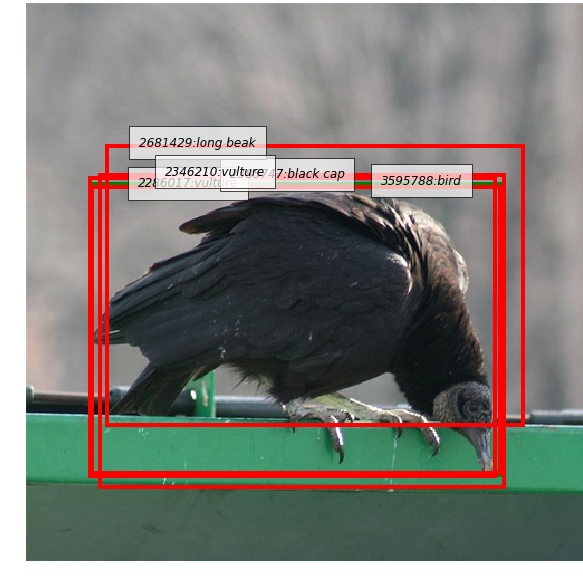
\includegraphics[scale=0.4]{figures/vulture.png} 
\begin{tabular}{lp{6cm}}
object id & linked region descriptions\\
\hline
3595788 & the \textbf{bird} is black in color, nose of the \textbf{bird}, a \textbf{bird} relaxing in stand, small white beak of \textbf{bird}, large black talon of \textbf{bird}, a \textbf{bird} on a green pole, a green bar under \textbf{bird}, black \textbf{bird} on green rail, small black eye of \textbf{bird}\\
2286017 & large black \textbf{vulture} on fence, a vulture on bar\\
2385747 & small white beak of \textbf{bird}\\
2681429 & a semi \textbf{long beak}\\  
2346210 & a black and gray \textbf{vulture}\\
 \end{tabular}
\caption{Bounding boxes, names and region descriptions for an object in VisualGenome}
\label{fig:bird}
\end{center}
\end{figure}

\vg \cite{krishna2016visualgenome} is one of the most densely and richly annotated resources currently available in L\&V; below, we focus on aspects immediately relevant to object naming.
%In the following, we will focus on describing aspects immediately relevant to object naming only, but many other annotations are available as well (e.g. questions, paragraphs, etc.)
%\paragraph{Collection and annotation procedure}
\vg aims at providing a full set of descriptions of the scenes which images depict in order to spur complete scene understanding. 
The data collection followed a complex procedure, involving many different rounds of annotation.
The first round of the procedure, and the basic backbone for the further rounds, is a collection of region-based descriptions: workers were asked to describe regions in the image and draw boxes around the corresponding area in the image (for examples, see Figure \ref{fig:bird}).

In a second, independent round (involving new workers), annotators were asked to process the region descriptions by (i) marking the object names contained in the region description, and (ii) drawing a tight box around the corresponding region. As different region descriptions can potentially mention the same objects, each worker was shown a list of previously marked objects and encouraged to select on existing object rather than annotating a new one.

\gbt{@Sina, pls check that I got this right:}
One of the main advantages of \vg are its size, with 3.8 million objects as opposed to 50K and 243K for the other two datasets, and its category coverage, with a vocabulary of object names of 105K compared to 5K/10K.
Another is the fact that it potentially provides exhaustive annotations of objects in the image, often with several region descriptions and possibly object names per object.
This should make it easier to identify factors intervening in naming choices.
However, there is a crucial pitfall: As Figure \ref{fig:bird} shows, there is only a partial linking of objects that are mentioned across different region descriptions; for instance, the first, second, and fifth object IDs in the figure actually correspond to the same object.
Moreover, the regions for the beak of the object (third and fourth object IDs) overlap with those of the bird.
This means that the identity of objects cannot be established based on the annotation, which severely limits the usefulness of the annotations.

\subsection{Discussion}

\gbt{Do we need a discussion section wrapping up what we've said in this survey section and motivating MN?}

As the discussion above showed, while some existing resources can be used to shed light on factors affecting naming choices, they do not provide enough data to assess \textbf{naming variation}, which requires having data from many subjects.
This is the motivation for our dataset, ManyNames, an augmentation of \vg.

%%% Local Variables:
%%% mode: latex
%%% TeX-master: "lrec2020naming"
%%% End:
